\documentclass[10pt, aspectratio=169, handout]{beamer}
\usefonttheme{professionalfonts}

\mode<presentation>{
  \usetheme{Berkeley}
  \usecolortheme{beaver}
  \usefonttheme{default}
  \setbeamertemplate{navigation symbols}{}
  \setbeamertemplate{caption}[numbered]
}

\setbeamertemplate{footline}{%
  \leavevmode%
  \hbox{%
    \begin{beamercolorbox}[wd=.85\paperwidth,ht=2.5ex,dp=1ex,left]{author in head/foot}%
      \usebeamerfont{author in head/foot}Digital Signal Processing, Fall 2025%
    \end{beamercolorbox}%
    \begin{beamercolorbox}[wd=.15\paperwidth,ht=2.5ex,dp=1ex,right]{date in head/foot}%
      \hspace*{0.5em}\insertframenumber{} / \inserttotalframenumber\hspace*{0.5em}%
    \end{beamercolorbox}%
  }%
  \vskip0pt%
}

\usepackage[english]{babel}
\usepackage[utf8]{inputenc}
\usepackage{tikz}
\usepackage{pgfplots}
\usepgfplotslibrary{groupplots}
\usetikzlibrary{calc, positioning, arrows.meta, backgrounds, plotmarks, shapes.geometric}
\pgfplotsset{compat=newest}

\usepackage{array}
\usepackage{makecell}
\usepackage{verbatim}
\usepackage{graphicx}
\usepackage{amsfonts}
\usepackage{amsmath}
\usepackage{bm}
\usepackage{epstopdf}
\usepackage[absolute,overlay]{textpos}
\usepackage{hyperref}
\hypersetup{colorlinks=true, linkcolor=blue, urlcolor=cyan}

\title[DSP]{Noise Shaping - Sigma Delta Modulation}
\author{Maxx Seminario}
\institute{University of Nebraska-Lincoln}
\date{Fall 2025}

\begin{document}

%--------------------------------------------------
\begin{frame}
  \titlepage
\end{frame}

%--------------------------------------------------
\section{Introduction and Motivation}

\begin{frame}{Why Oversampling?}
\small

\textbf{Key Concept:} Sample at a rate \emph{higher} than the Nyquist rate to gain advantages in A/D and D/A conversion.

\vspace{0.3cm}
\textbf{Benefits:}
\begin{itemize}
  \item \textbf{Simplified Antialiasing Filters:} Oversampling relaxes analog filter requirements
  \item \textbf{Reduced Quantization Noise:} Spreading noise over wider bandwidth
  \item \textbf{Increased Effective Resolution:} Can achieve high bit accuracy with coarse quantizers
  \item \textbf{Cost-Effective Design:} Trade computation for analog precision
\end{itemize}

\vspace{0.3cm}
\textbf{Applications:}
\begin{itemize}
  \item High-quality audio (CD, DAC)
  \item Precision measurement systems
  \item Software-defined radio
\end{itemize}

\end{frame}

%--------------------------------------------------
\begin{frame}{Oversampling Ratio}
\small

\textbf{Definition:} The \textbf{oversampling ratio} $M$ is:
\[
M = \frac{f_s}{2f_N}
\]
where:
\begin{itemize}
  \item $f_s$ = actual sampling frequency
  \item $f_N$ = Nyquist frequency (bandwidth of signal)
\end{itemize}

\vspace{0.3cm}
\textbf{Key Idea:} As $M$ increases, we can:
\begin{itemize}
  \item Reduce quantizer bits
  \item Improve signal-to-noise ratio (SNR)
  \item Use digital filtering to remove out-of-band noise
\end{itemize}

\end{frame}

%--------------------------------------------------
\begin{frame}{System Overview: Direct Quantization}
\small

\textbf{Basic System:}

\vspace{0.4cm}
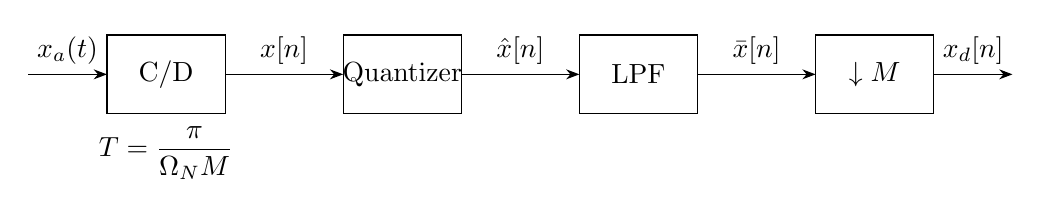
\begin{tikzpicture}[>=Stealth]

  % Blocks
  \draw (0,0) rectangle (1.5,1) node[midway] {C/D};
  \draw (3,0) rectangle (4.5,1) node[midway] {Quantizer};
  \draw (6,0) rectangle (7.5,1) node[midway] {LPF};
  \draw (9,0) rectangle (10.5,1) node[midway] {$\downarrow M$};

  % Arrows and labels
  \draw[->] (-1,0.5) -- (0,0.5) node[midway, above] {$x_a(t)$};
  \draw[->] (1.5,0.5) -- (3,0.5) node[midway, above] {$x[n]$};
  \draw[->] (4.5,0.5) -- (6,0.5) node[midway, above] {$\hat{x}[n]$};
  \draw[->] (7.5,0.5) -- (9,0.5) node[midway, above] {$\bar{x}[n]$};
  \draw[->] (10.5,0.5) -- (11.5,0.5) node[midway, above] {$x_d[n]$};

  % Text below C/D block
  \node at (0.75,-0.5) {$T = \dfrac{\pi}{\Omega_N M}$};

\end{tikzpicture}

\vspace{0.3cm}
\textbf{Process:}
\begin{enumerate}
  \item Sample at high rate: $T = \pi/(\Omega_N M)$
  \item Quantize samples
  \item Lowpass filter to remove out-of-band noise
  \item Downsample by $M$ to return to Nyquist rate
\end{enumerate}

\end{frame}

%--------------------------------------------------
\begin{frame}{Additive Noise Model}
\small

\textbf{Quantizer Model:} Replace quantizer with additive white noise

\vspace{0.4cm}
\begin{center}
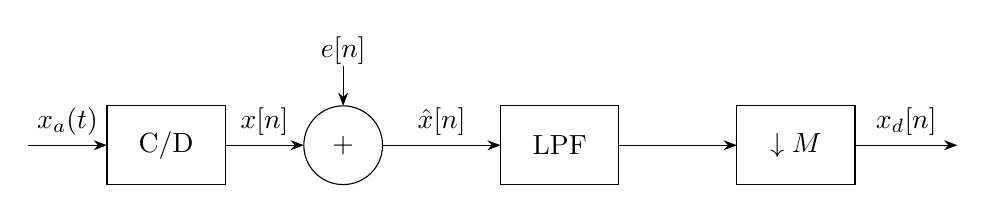
\begin{tikzpicture}[>=Stealth]

  % Blocks
  \draw (0,0) rectangle (1.5,1) node[midway] {C/D};
  \draw (3,0.5) circle (0.5) node {$+$};
  \draw (5,0) rectangle (6.5,1) node[midway] {LPF};
  \draw (8,0) rectangle (9.5,1) node[midway] {$\downarrow M$};

  % Main signal path
  \draw[->] (-1,0.5) -- (0,0.5) node[midway, above] {$x_a(t)$};
  \draw[->] (1.5,0.5) -- (2.5,0.5) node[midway, above] {$x[n]$};
  \draw[->] (3.5,0.5) -- (5,0.5) node[midway, above] {$\hat{x}[n]$};
  \draw[->] (6.5,0.5) -- (8,0.5);
  \draw[->] (9.5,0.5) -- (10.8,0.5) node[midway, above] {$x_d[n]$};

  % Noise input
  \node at (3,1.7) {$e[n]$};
  \draw[->] (3,1.5) -- (3,1);

\end{tikzpicture}
\end{center}

\vspace{0.3cm}
\textbf{Noise Properties:}
\begin{itemize}
  \item White noise: $\phi_{ee}[m] = \sigma_e^2 \delta[m]$
  \item Uniform distribution over quantization step $\Delta$
  \item Variance: $\sigma_e^2 = \dfrac{\Delta^2}{12}$
  \item Power spectral density: $\Phi_{ee}(e^{j\omega}) = \sigma_e^2$ for $|\omega| < \pi$
\end{itemize}

\end{frame}

%--------------------------------------------------
\begin{frame}{Signal and Noise Power Analysis}
\small

\textbf{Signal Power:} Remains constant throughout processing
\[
E\{x_a^2(t)\} = E\{x^2[n]\} = E\{x_{d}^2[n]\}
\]

\vspace{0.3cm}
\textbf{Quantization Noise Power:}

Before filtering:
\[
E\{e^2[n]\} = \sigma_e^2 = \frac{\Delta^2}{12}
\]

After lowpass filtering and decimation:
\[
E\{x_{de}^2[n]\} = \frac{1}{2\pi} \int_{-\pi/M}^{\pi/M} \sigma_e^2 \, d\omega = \frac{\sigma_e^2}{M} = \frac{\Delta^2}{12M}
\]

\vspace{0.2cm}
\textbf{Key Result:} Noise power reduced by factor of $M$!

\end{frame}

%--------------------------------------------------
\begin{frame}{Power Spectral Density Illustration}
\small

\begin{center}
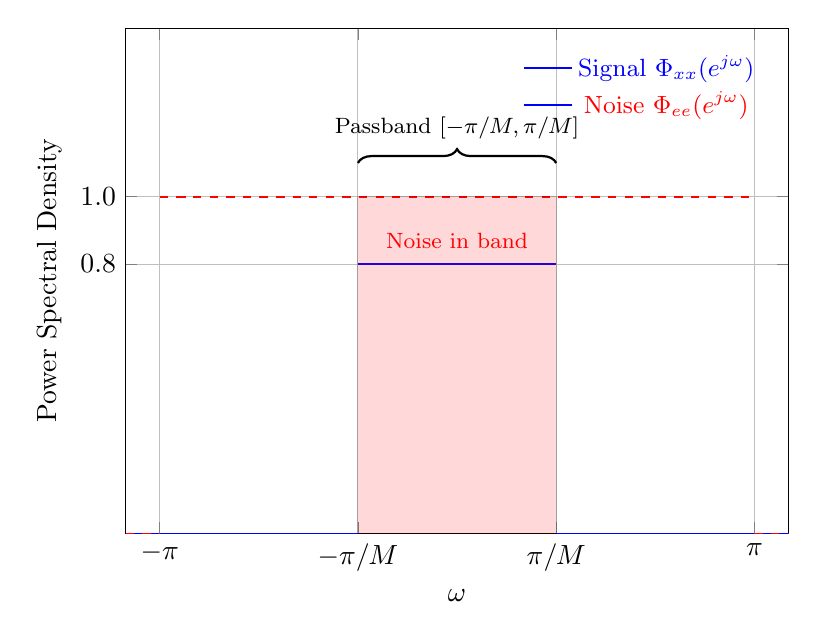
\begin{tikzpicture}[scale=1.0]
  % Signal and noise spectrum
  \begin{axis}[
    width=10cm, height=8cm,
    xlabel={$\omega$},
    ylabel={Power Spectral Density},
    xmin=-3.5, xmax=3.5,
    ymin=0, ymax=1.5,
    xtick={-3.14, -1.047, 1.047, 3.14},
    xticklabels={$-\pi$, $-\pi/M$, $\pi/M$, $\pi$},
    ytick={0.8, 1.0},
    yticklabels={$0.8$, $1.0$},
    legend pos=north east,
    grid=major,
    legend style={draw=none, fill=none, font=\small}
  ]
  
  % Signal band
  \addplot[thick, blue, domain=-1.047:1.047] {0.8};
  % Zero elsewhere for signal
  \addplot[thick, blue] coordinates {(-3.5,0) (-1.047,0)};
  \addplot[thick, blue] coordinates {(1.047,0) (3.5,0)};
  
  % Noise spectrum, everywhere
  \addplot[thick, red, dashed, domain=-3.14:3.14] {1.0};
  \addplot[thick, red, dashed] coordinates {(-3.5,0) (-3.14,0)};
  \addplot[thick, red, dashed] coordinates {(3.14,0) (3.5,0)};
  
  % Shaded region for noise inside signal band
  \addplot[fill=red, opacity=0.15, domain=-1.047:1.047] {1.0} \closedcycle;
  
  % Legend with clear text and color matching
  \legend{
    {\color{blue} Signal $\Phi_{xx}(e^{j\omega})$}, 
    {\color{red} Noise $\Phi_{ee}(e^{j\omega})$}
  }
  
  % Annotation: filtered band
  % \node[anchor=south east, font=\footnotesize] at (axis cs: -1.047,1.08) {Signal Band};
  % \node[anchor=south west, font=\footnotesize] at (axis cs: 1.047,1.08) {Signal Band};
  \draw [black, thick, decorate,decoration={brace,amplitude=5pt}]
    (axis cs:-1.047,1.1) -- (axis cs:1.047,1.1) node[midway,above=5pt, font=\footnotesize]{Passband $[-\pi/M, \pi/M]$};

  % Optionally, annotate the shaded region as "Noise remains"
  \node[anchor=north, font=\footnotesize, color=red] at (axis cs: 0,0.92) {Noise in band};

  \end{axis}
\end{tikzpicture}
\end{center}

% \textbf{Observation:} Only noise in signal band $[-\pi/M, \pi/M]$ remains after filtering.

% \vspace{0.2em}
% {\scriptsize \textbf{Legend:} \color{blue}Solid blue line = Signal spectrum, \color{red} dashed red line = Noise spectrum, \color{red!50} shaded = Noise that remains in the signal band}

\end{frame}

%--------------------------------------------------
\begin{frame}{Bit Reduction Trade-off}
\small

\textbf{Quantizer Step Size:} For $(B+1)$-bit quantizer with maximum input $\pm X_m$:
\[
\Delta = \frac{X_m}{2^B}
\]

\textbf{Output Noise Power:}
\[
P_{de} = E\{x_{de}^2[n]\} = \frac{1}{12M} \left(\frac{X_m}{2^B}\right)^2
\]

\textbf{Required Bits for Given Noise Power:}
\[
B = -\frac{1}{2}\log_2 M - \frac{1}{2}\log_2(12) - \frac{1}{2}\log_2 P_{de} + \log_2 X_m
\]

\vspace{0.2cm}
Every doubling of oversampling ratio $M$ saves \textbf{0.5 bits} of quantization!

\end{frame}

%--------------------------------------------------
\begin{frame}{Example: Bit Savings}
\small

\textbf{Question:} How much oversampling is needed to use a 12-bit quantizer instead of a 16-bit quantizer, while maintaining the same effective noise performance?

\vspace{0.3cm}
\textbf{Solution:}
\begin{itemize}
  \item Bit reduction needed: $16 - 12 = 4$ bits
  \item Each doubling of $M$ saves 0.5 bit
  \item Doublings needed: $4 / 0.5 = 8$
  \item Required oversampling: $M = 2^8 = 256$
\end{itemize}

\vspace{0.3cm}
\textbf{Practical Consideration:}
\begin{itemize}
  \item $M = 256$ is too high for many applications
  \item Need better approach $\rightarrow$ \textbf{Noise Shaping}
\end{itemize}

\end{frame}

%--------------------------------------------------
\section{Noise Shaping: Delta-Sigma Modulation}

\begin{frame}{Motivation for Noise Shaping}
\small

\textbf{Problem with Direct Quantization:}
\begin{itemize}
  \item Quantization noise has \emph{flat} spectrum
  \item All frequencies equally contaminated
  \item Need high $M$ for significant bit reduction
\end{itemize}

\vspace{0.3cm}
\textbf{Better Idea: Noise Shaping}
\begin{itemize}
  \item \textbf{Shape} the noise spectrum using feedback
  \item Push noise power to \emph{high frequencies}
  \item More noise removed by lowpass filter
  \item Same $M$ gives better performance
\end{itemize}

\vspace{0.3cm}
\begin{block}{Core Concept}
Use feedback to make quantization error spectrum non-uniform, concentrating noise outside the signal band.
\end{block}

\end{frame}

%--------------------------------------------------
\begin{frame}{First-Order Delta-Sigma Modulator}
\small

\textbf{System Structure:}

\vspace{0.2cm}
\begin{center}
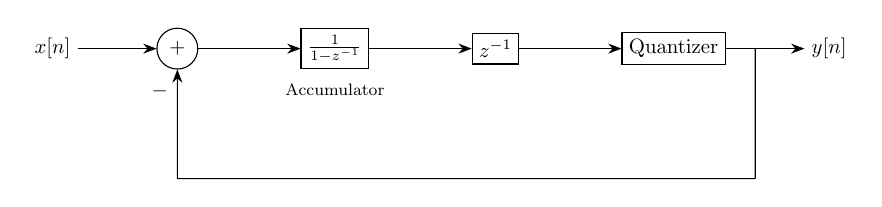
\begin{tikzpicture}[>=Stealth, node distance=1.3cm, scale=0.75, every node/.style={scale=0.75}]
  % Input
  \node (input) {$x[n]$};
  
  % First summer: plus over minus style
  \node[draw, circle, right=1cm of input] (sum1) {$+$};
  % Alternatively, {$+\!\!-\:$} for tighter layout

  \node[below=0.1cm of sum1, xshift=-0.3cm] {$-$};

  % Integrator
  \node[draw, rectangle, right=of sum1] (int) {$\frac{1}{1-z^{-1}}$};
  
  % Delay
  \node[draw, rectangle, right=of int] (delay) {$z^{-1}$};
  
  % Quantizer
  \node[draw, rectangle, right=of delay] (quant) {Quantizer};
  
  % Output
  \node[right=1cm of quant] (output) {$y[n]$};
  
  % Feedback path: make a coordinate directly below sum1
  \coordinate (fb1) at ($(quant.east)+(0.5,0)$);
  \coordinate (fb2) at ($(fb1)+(0,-2.2)$);
  \coordinate (fb3) at ($(sum1)+(0,-2.2)$);
  
  % Connections
  \draw[->] (input) -- (sum1);
  \draw[->] (sum1) -- (int);
  \draw[->] (int) -- (delay);
  \draw[->] (delay) -- (quant);
  \draw[->] (quant) -- (output);
  
  % Feedback
  \draw[->] (fb1) |- (fb2) -| (fb3) -- (sum1.south);

  % Labels
  \node[below=0.1cm of int] {\footnotesize Accumulator};
\end{tikzpicture}
\end{center}

\vspace{0.2cm}
\textbf{Also known as:}
\begin{itemize}
  \item Delta-Sigma ($\Delta\Sigma$) modulator
  \item Sigma-Delta ($\Sigma\Delta$) modulator
  \item 1-bit ADC with noise shaping
\end{itemize}

\end{frame}

%--------------------------------------------------
\begin{frame}{Linear Noise Model Analysis}
\small

\textbf{Replace quantizer with additive noise:}

% \vspace{0.2cm}
\begin{center}
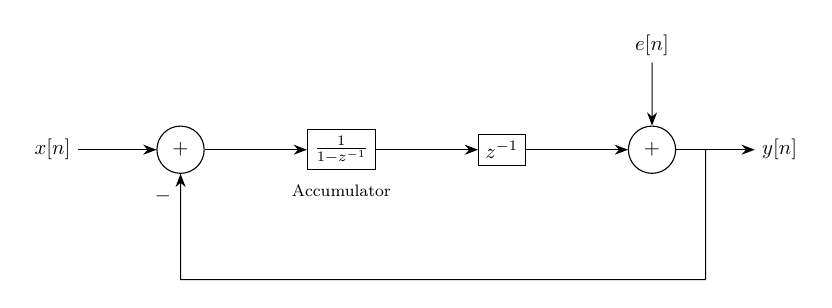
\begin{tikzpicture}[>=Stealth, node distance=1.3cm, scale=0.75, every node/.style={scale=0.75}]
  % Input
  \node (input) {$x[n]$};

  % First summer: plus with minus below and left
  \node[draw, circle, right=1cm of input, minimum size=0.8cm] (sum1) {$+$};
  \node[below=0.1cm of sum1, xshift=-0.3cm] {$-$};

  % Integrator
  \node[draw, rectangle, right=of sum1] (int) {$\frac{1}{1-z^{-1}}$};

  % Delay
  \node[draw, rectangle, right=of int] (delay) {$z^{-1}$};

  % Second summer and noise
  \node[draw, circle, right=of delay, minimum size=0.8cm] (sum2) {$+$};
  \node[above=0.8cm of sum2] (noise) {$e[n]$};

  % Output
  \node[right=1cm of sum2] (output) {$y[n]$};

  % Feedback path coordinates
  \coordinate (fb1) at ($(sum2.east)+(0.5,0)$);
  \coordinate (fb2) at ($(fb1)+(0,-2.2)$);
  \coordinate (fb3) at ($(sum1)+(0,-2.2)$);

  % Connections
  \draw[->] (input) -- (sum1);
  \draw[->] (sum1) -- (int);
  \draw[->] (int) -- (delay);
  \draw[->] (delay) -- (sum2);
  \draw[->] (noise) -- (sum2);
  \draw[->] (sum2) -- (output);

  % Feedback path
  \draw[->] (fb1) |- (fb2) -| (fb3) -- (sum1.south);

  % Label
  \node[below=0.1cm of int] {\footnotesize Accumulator};
\end{tikzpicture}
\end{center}

% \vspace{0.3cm}
\textbf{Transfer Functions:}

Signal path:
\[
H_x(z) = \frac{Y(z)}{X(z)}\bigg|_{e[n]=0} = 1
\]

Noise path:
\[
H_e(z) = \frac{Y(z)}{E(z)}\bigg|_{x[n]=0} = 1 - z^{-1}
\]

\end{frame}

%--------------------------------------------------
\begin{frame}{Noise Shaping Effect}
\small

\textbf{Output:}
\[
y[n] = x[n] + \hat{e}[n]
\]
where $\hat{e}[n] = e[n] - e[n-1]$ (first difference of quantization noise)

\vspace{0.3cm}
\textbf{Noise Power Spectrum:}
\[
\Phi_{\hat{e}\hat{e}}(e^{j\omega}) = \sigma_e^2 |H_e(e^{j\omega})|^2 = \sigma_e^2 |1 - e^{-j\omega}|^2 = \sigma_e^2 \cdot 4\sin^2(\omega/2)
\]

\vspace{0.3cm}
\textbf{Key Properties:}
\begin{itemize}
  \item At DC ($\omega = 0$): $\Phi_{\hat{e}\hat{e}}(1) = 0$ (noise suppressed)
  \item At Nyquist ($\omega = \pi$): $\Phi_{\hat{e}\hat{e}}(e^{j\pi}) = 4\sigma_e^2$ (noise amplified)
  \item Total noise power: $E\{\hat{e}^2[n]\} = 2\sigma_e^2$ (increased from $\sigma_e^2$)
  \item But most noise is at high frequencies
\end{itemize}

\end{frame}

%--------------------------------------------------
\begin{frame}{Shaped Noise Spectrum}
\small

\begin{center}
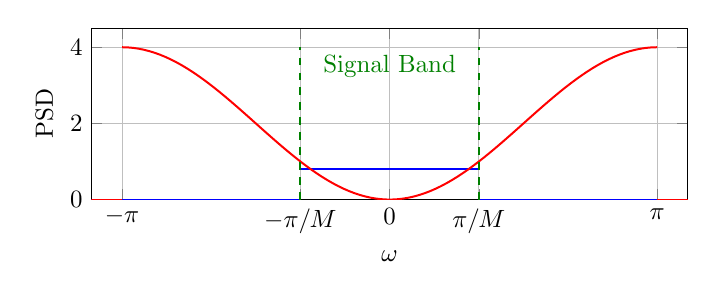
\begin{tikzpicture}[scale=0.9]
  \begin{axis}[
    width=10cm, height=4cm,
    xlabel={$\omega$},
    ylabel={PSD},
    xmin=-3.5, xmax=3.5,
    ymin=0, ymax=4.5,
    xtick={-3.14, -1.047, 0, 1.047, 3.14},
    xticklabels={$-\pi$, $-\pi/M$, $0$, $\pi/M$, $\pi$},
    legend pos=north west,
    grid=major
  ]
  
  % Signal spectrum
  \addplot[thick, blue, domain=-1.047:1.047] {0.8};
  \addplot[thick, blue] coordinates {(-3.5,0) (-1.047,0)};
  \addplot[thick, blue] coordinates {(1.047,0) (3.5,0)};
  
  % Shaped noise spectrum
  \addplot[thick, red, domain=-3.14:3.14, samples=100] {4*sin(deg(x/2))^2};
  \addplot[thick, red] coordinates {(-3.5,0) (-3.14,0)};
  \addplot[thick, red] coordinates {(3.14,0) (3.5,0)};
  
  % \legend{Signal, Shaped Noise}
  
  % Highlight signal band
  \draw[thick, green!50!black, dashed] (-1.047,0) -- (-1.047,4);
  \draw[thick, green!50!black, dashed] (1.047,0) -- (1.047,4);
  
  \node[green!50!black] at (0, 3.5) {Signal Band};
  
  \end{axis}
\end{tikzpicture}
\end{center}

\textbf{Result:} Much less noise in signal band compared to flat spectrum

\end{frame}

%--------------------------------------------------
\begin{frame}{Noise Power After Decimation}
\small

\textbf{After lowpass filtering and downsampling:}

\[
P_{de} = \frac{1}{2\pi} \int_{-\pi/M}^{\pi/M} \sigma_e^2 \cdot 4\sin^2(\omega/2) \, d\omega
\]

\textbf{For large $M$:} $\sin(\omega/2M) \approx \omega/2M$

\[
P_{de} \approx \frac{1}{2\pi} \int_{-\pi/M}^{\pi/M} \sigma_e^2 \cdot \left(\frac{\omega}{M}\right)^2 d\omega = \frac{\sigma_e^2 \pi^2}{12M^3} = \frac{\Delta^2}{12} \cdot \frac{\pi^2}{M^3}
\]

\vspace{0.3cm}
\textbf{Bit requirement:}
\[
B = -\frac{3}{2}\log_2 M + \log_2(\pi/\sqrt{6}) - \frac{1}{2}\log_2 P_{de} + \log_2 X_m
\]

\vspace{0.2cm}
% \begin{block}{Key Result}
\textbf{Result:} Every doubling of $M$ saves \textbf{1.5 bits} (vs. 0.5 bits without noise shaping)
% \end{block}

\end{frame}

%--------------------------------------------------
\begin{frame}{Comparison: Direct vs. Noise Shaping}
\small

\begin{center}
\begin{tabular}{|c|c|c|}
\hline
\textbf{Oversampling} & \textbf{Direct} & \textbf{1st-Order} \\
\textbf{Ratio $M$} & \textbf{Quantization} & \textbf{Noise Shaping} \\
\hline
4 & 1.0 & 2.2 \\
8 & 1.5 & 3.7 \\
16 & 2.0 & 5.1 \\
32 & 2.5 & 6.6 \\
64 & 3.0 & 8.1 \\
\hline
\end{tabular}
\end{center}

\vspace{0.2cm}
\textbf{Equivalent Bit Savings} (relative to no oversampling)

\vspace{0.3cm}
\textbf{Example:} With $M = 64$:
\begin{itemize}
  \item Direct: 3 extra bits $\rightarrow$ 13-bit effective from 16-bit quantizer
  \item Noise shaping: 8.1 extra bits $\rightarrow$ \textbf{8-bit effective from 16-bit quantizer}
\end{itemize}

\end{frame}

%--------------------------------------------------

\section{Higher-Order Noise Shaping}
\begin{frame}{Second-Order Delta-Sigma Modulator}
\small

\textbf{Add another integrator stage:}

\vspace{0.2cm}
\begin{center}
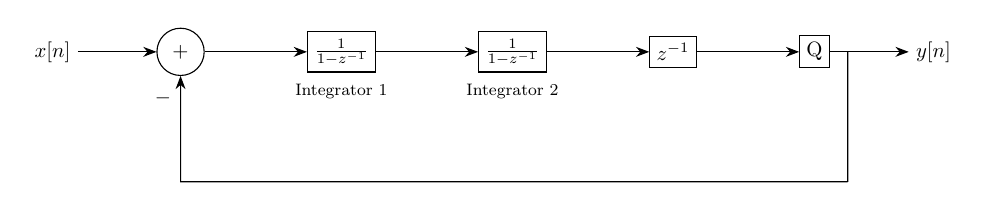
\begin{tikzpicture}[>=Stealth, node distance=1.3cm, scale=0.75, every node/.style={scale=0.75}]
  % Input
  \node (input) {$x[n]$};
  
  % First summer
  \node[draw, circle, right=1cm of input, minimum size=0.8cm] (sum1) {$+$};
  \node[below=0.1cm of sum1, xshift=-0.3cm] {$-$};
  
  % First integrator
  \node[draw, rectangle, right=of sum1] (int1) {$\frac{1}{1-z^{-1}}$};
  
  % Second integrator (no summer between them!)
  \node[draw, rectangle, right=of int1] (int2) {$\frac{1}{1-z^{-1}}$};
  
  % Delay
  \node[draw, rectangle, right=of int2] (delay) {$z^{-1}$};
  
  % Quantizer
  \node[draw, rectangle, right=of delay] (quant) {Q};
  
  % Output
  \node[right=1cm of quant] (output) {$y[n]$};
  
  % Single feedback path (from output to first summer)
  \coordinate (fb1) at ($(quant.east)+(0.3,0)$);
  \coordinate (fb2) at ($(fb1)+(0,-2.2)$);
  \coordinate (fb3) at ($(sum1)+(0,-2.2)$);
  
  % Forward connections
  \draw[->] (input) -- (sum1);
  \draw[->] (sum1) -- (int1);
  \draw[->] (int1) -- (int2);
  \draw[->] (int2) -- (delay);
  \draw[->] (delay) -- (quant);
  \draw[->] (quant) -- (output);
  
  % Single feedback path
  \draw[->] (fb1) |- (fb2) -| (fb3) -- (sum1.south);
  
  % Labels
  \node[below=0.05cm of int1] {\footnotesize Integrator 1};
  \node[below=0.05cm of int2] {\footnotesize Integrator 2};
  
\end{tikzpicture}
\end{center}

\vspace{0.3cm}
\textbf{Noise Transfer Function:}
\[
H_e(z) = (1 - z^{-1})^2
\]

\textbf{Shaped Noise PSD:}
\[
\Phi_{\hat{e}\hat{e}}(e^{j\omega}) = \sigma_e^2 \cdot 16\sin^4(\omega/2)
\]

Even stronger high-frequency emphasis!

\end{frame}


%--------------------------------------------------
\begin{frame}{General $p$-th Order Noise Shaping}
\small

\textbf{Order $p$ modulator:}
\[
H_e(z) = (1 - z^{-1})^p
\]

\textbf{Noise PSD:}
\[
\Phi_{\hat{e}\hat{e}}(e^{j\omega}) = \sigma_e^2 \cdot [2\sin(\omega/2)]^{2p}
\]

\textbf{Noise power (large $M$ approximation):}
\[
P_{de} \approx \frac{\sigma_e^2 \pi^{2p}}{(2p+1)M^{2p+1}}
\]

\vspace{0.2cm}
\begin{block}{Scaling Law}
Order $p$ noise shaping: doubling $M$ saves $(p + 0.5)$ bits
\begin{itemize}
  \item $p=0$ (direct): 0.5 bits per doubling
  \item $p=1$: 1.5 bits per doubling
  \item $p=2$: 2.5 bits per doubling
\end{itemize}
\end{block}

\end{frame}

%--------------------------------------------------
\begin{frame}{Performance Comparison Table}
\small

\textbf{Bit reduction relative to no oversampling:}

\vspace{0.2cm}
\begin{center}
\begin{tabular}{|c|c|c|c|c|c|}
\hline
\textbf{Order} & \multicolumn{5}{c|}{\textbf{Oversampling Factor $M$}} \\
\cline{2-6}
$p$ & 4 & 8 & 16 & 32 & 64 \\
\hline
0 & 1.0 & 1.5 & 2.0 & 2.5 & 3.0 \\
1 & 2.2 & 3.7 & 5.1 & 6.6 & 8.1 \\
2 & 2.9 & 5.4 & 7.9 & 10.4 & 12.9 \\
3 & 3.5 & 7.0 & 10.5 & 14.0 & 17.5 \\
4 & 4.1 & 8.5 & 13.0 & 17.5 & 22.0 \\
\hline
\end{tabular}
\end{center}

\vspace{0.3cm}
\textbf{Remarkable Example:}
\begin{itemize}
  \item 2nd-order, $M=64$: 12.9 bit improvement
  \item Can achieve 14-bit accuracy with \textbf{1-bit quantizer}!
  \item (16 bits - 12.9 bits $\approx$ 3 bits $\rightarrow$ use simple comparator)
\end{itemize}

\end{frame}

%--------------------------------------------------
\begin{frame}{Practical Considerations}
\small

\textbf{Advantages of Higher-Order Modulators:}
\begin{itemize}
  \item Dramatic improvement in resolution
  \item Can use very simple (1-bit) quantizers
  \item Excellent linearity
\end{itemize}

\vspace{0.3cm}
\textbf{Challenges:}
\begin{itemize}
  \item \textbf{Stability:} Higher-order loops can oscillate
  \item \textbf{Overload:} Large signals can cause instability
  \item Require careful design and analysis
\end{itemize}

\vspace{0.3cm}
\textbf{Alternative: MASH (Multi-stAge noise SHaping)}
\begin{itemize}
  \item Cascade multiple 1st-order stages
  \item Each stage shapes the previous stage's quantization error
  \item More stable than single high-order loop
\end{itemize}

\end{frame}

%-------

\end{document}